% !TeX encoding = UTF-8
% Lecture file created by newnote
% Class: Models of Theoretical Physics
% Professor: Azaele Sandro
% Date: 2025-10-17
\lecture{3}{Fokker-Planck equation derivation}{2025-10-17}
\pagelayout{margin}
% --- Start writing here ---

\section{Fokker-Planck equation derivation}
Derivation of the Fokker-Planck equation for a general Langevin equation (Itô
prescription)

We start from a stochastic process defined via the Langevin equation (Itô)
\begin{DispWithArrows}[displaystyle, format=c]
  d x(t)=\mu(x(t), t) d t+\sigma(x(t), t) d B(t)
\end{DispWithArrows}
where $x(0)=x_{0}$ (or a generic initial PDF). $B(t)$ is a standard Brownian
process.
An alternative way to write eq. (1) is the "pseudo-equation"
\begin{DispWithArrows}[displaystyle, format=c]
  \dot{x}=\mu(x, t)+\sigma(x, t) \xi(t)
\end{DispWithArrows}
Where $\langle\xi(t)\rangle=0$ and
$\left\langle\xi\left(t^{\prime}\right) \xi(t)\right\rangle=\delta\left(t^{\prime}-t\right)$.
We used the suggestive relation " $\frac{d B}{d t}=\xi$ ", even though this is
only a formal, notational expression.

Eq. (1) defines the process $x(t)$ so we can use the eq. to generate as many
trajectories as we wish. Let us assume that we have generated a large number $N$
of paths from time $t=0$ to $t=T>0$. How can we calculate the probability that
$x(t)$ gets a value between $x$ and $x+\Delta x$ (a PDF) at time $t$?

From the computational point of view this is relatively easy:
\begin{figure}[H]
    \centering
    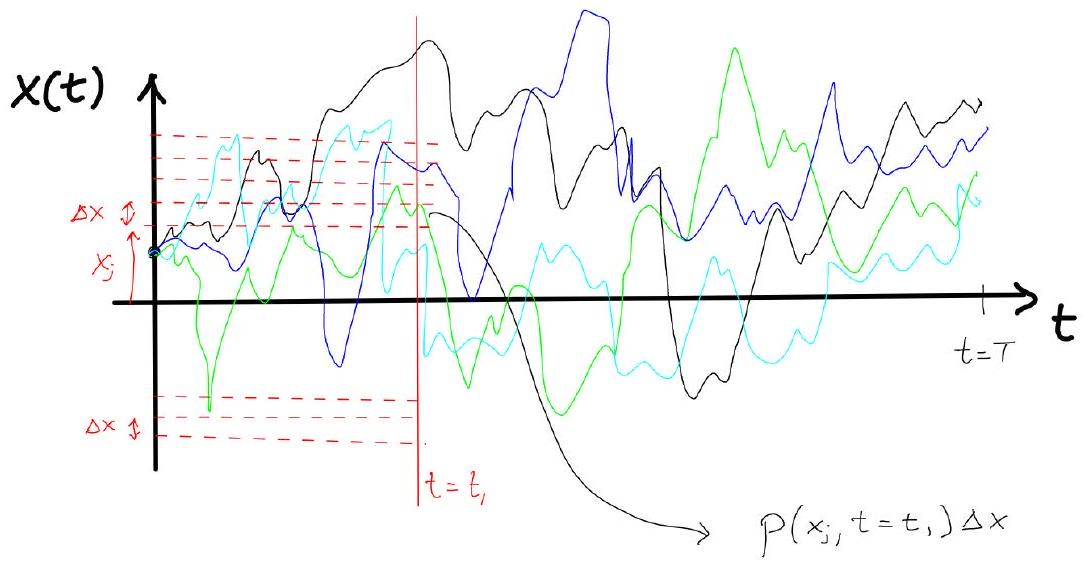
\includegraphics[width=\textwidth]{graphics/2025_10_17_1e406b49946272086d2dg-02}
\end{figure}
We have to count how many paths fall in the interval $[x, x+\Delta x)$ at time
$t=t_{1}$ as $x$ varies in the domain of definition of the process $x(t)$.
If we use the indicator function, $I$, defined as
\begin{DispWithArrows}[displaystyle, format=ll]
  I(a, A)= \left\{\begin{aligned}1 & a \in A \\ 0 & a \notin A\end{aligned}\right.
\end{DispWithArrows}
then we calculate numerically $P(x, t)$ as
\begin{DispWithArrows}[displaystyle, format=c]
  P\left(x_{j}, t=t_{1}\right) \Delta x=\lim _{N \rightarrow \infty} \frac{1}{N} \sum_{1}^{N} I\left(x^{i}\left(t_{1}\right),\left[x_{j}, x_{j}+\Delta x\right)\right)
\end{DispWithArrows}
for any $x_{j}$ and various $t$.

Where $x_{j}=j \Delta x$ and
$j=j_{\min }, j_{\min }+1, \ldots j_{\max }-1, j_{\max }$ (uniform mesh). For
example, if the process was Brownian, then $P(x, t)$ would be very well
approximated by a Gaussian distribution with zero mean and variance $t$, as we
saw before. Notice that if we say $x_{j}=x, t=t$, and take the limit
$\Delta x \rightarrow 0$, then
\begin{DispWithArrows}[displaystyle, format=c]
  P(x, t)=\lim _{N \rightarrow \infty} \frac{1}{N} \sum_{i}^{N} \delta\left(x-x_{i}(t)\right) \text { as } \lim _{\Delta x \rightarrow 0} \frac{I\left(x^{i}(t),[x, x+\Delta x)\right)}{\Delta x}=\delta\left(x-x_{i}(t)\right)
\end{DispWithArrows}
From the theoretical point of view we want to find out an equation for $P(x, t)$
which gives the PDF of the process $x(t)$. If we are interested in the
statistics of the process, then $P(x, t)$ gives all the information we need, for
we can calculate all averages we want (all moments) (even though it is not
guaranteed that from the PDF we can exactly reconstruct the process $x(t)$
pathwise).
Actually, we can calculate the average of any "sufficiently regular" function
$f$.
Let's assume that $f$ has compact support in $\mathbb{R}$ and is
twice-differentiable, namely $f \in C_{c}^{2}(\mathbb{R})$.
Then we can calculate $\langle f(x(t))\rangle$, average of $f$ over the process.
If we are given $N$ indep. realizations of $x(t)$, then as $N \rightarrow \infty$
\begin{DispWithArrows}[displaystyle, format=c]
  $\langle f(x(t))\rangle=\lim _{N} \frac{1}{N} \sum_{i}^{N} f\left(x_{i}(t)\right)=\lim _{N} \frac{1}{N} \sum_{i}^{N} \int d x f(x) \delta\left(x-x_{i}(t)\right) = \int d x f(x) \lim _{N} \frac{1}{N} \sum_{i}^{N} \delta\left(x-x_{i}(t)\right) \stackrel{\downarrow}{=} \int d x f(x) p(x, t)$
\end{DispWithArrows}
Hence
\begin{DispWithArrows}[displaystyle, format=c]
  $\frac{d}{d t}\langle f(x(t))\rangle \equiv \int \dot{p}(x, t) f(x) d x$
\end{DispWithArrows}
Here $\langle\cdots\rangle$ means that the average of $f$ has to be calculated
over the whole set of trajectories of the process $x(t)$. We now discretize the
process in time and Taylor-expand the function $f(x)$:
\begin{DispWithArrows}[displaystyle, format=c]
  $f(x(t+\Delta t))=f(x(t))+\Delta x f^{\prime}(x(t))+\frac{\Delta x^{2}}{2} f^{\prime \prime}(x(t))+\text { h.o.t. }$
\end{DispWithArrows}
where from eq. (1) we get
\begin{DispWithArrows}[displaystyle, format=c]
  $\Delta x \equiv x(t+\Delta t)-x(t)=\mu(x(t), t) \Delta t+\sigma(x(t), t) \Delta B(t)$ 
\end{DispWithArrows}
Therefore from (6) $\Delta f \equiv f(x(t+\Delta t))-f(x(t))$
\begin{DispWithArrows}[displaystyle, format=ll]
  \begin{aligned}
    &\Delta f &=f^{\prime}(\mu \Delta t+\sigma \Delta B)+\frac{1}{2} f^{\prime \prime}(\mu \Delta t+\sigma \Delta B)^{2}+\text { h.o.t. } \\
    & &=f^{\prime}(\mu \Delta t+\sigma \Delta B)+\frac{1}{2} f^{\prime \prime}\left(\mu^2\Delta t^2+2 \mu \sigma \Delta t \Delta B+\sigma^{2} \Delta B^{2}\right)+\text { h.o.t. }
  \end{aligned}
\end{DispWithArrows}
We now consider the average of each term:
a)
$\left\langle f^{\prime} \sigma \Delta B\right\rangle=\left\langle f^{\prime} \sigma\right\rangle\langle\Delta B\rangle=0$
(Itô prescription)
b)
$\left\langle f^{\prime \prime} \mu \sigma \Delta t \Delta B\right\rangle=\left\langle f^{\prime \prime} \mu \sigma\right\rangle \Delta t\langle\Delta B\rangle=0$
c)
$\frac{1}{2}\left\langle f^{\prime \prime} \sigma^{2} \Delta B^{2}\right\rangle=\frac{1}{2}\left\langle f^{\prime \prime} \sigma^{2}\right\rangle\left\langle\Delta B^{2}\right\rangle=\frac{1}{2}\left\langle f^{\prime \prime} \sigma^{2}\right\rangle \Delta t$
(Itô preser. IMPORTANT!)
all remaining terms are $O\left(\Delta t^{2}\right)$.
Therefore eq. (5) can be re-written as limit
\begin{DispWithArrows}[displaystyle, format=c]
  $\lim _{\Delta t \rightarrow 0}\left\langle\frac{\Delta f}{\Delta t}\right\rangle=\left\langle f^{\prime} \mu\right\rangle+\frac{1}{2}\left\langle f^{\prime \prime} \sigma^{2}\right\rangle = \int d x p(x, t)\left[f^{\prime}(x) \mu(x, t)+\frac{1}{2} f^{\prime \prime}(x) \sigma^{2}(x, t)\right]$
\end{DispWithArrows}
As $f \in C_{c}^{2}(\mathbb{R})$ we can integrate by parts and safely assume
that $f, f^{\prime}$ and $f^{\prime \prime} \rightarrow 0$ as $|x|$ is large
enough. Hence
\begin{DispWithArrows}[displaystyle, format=c]
  $\int d x p(x, t) \mu(x, t) \frac{\partial f}{\partial x} \stackrel{\downarrow}{=}-\int d x f(x) \frac{\partial}{\partial x}(p \mu)$
\end{DispWithArrows}
twice integrated by parts
\begin{DispWithArrows}[displaystyle, format=c]
  $\int d x p(x, t) \frac{\sigma^{2}(x, t)}{2} \frac{\partial^{2} f}{\partial x^{2}}=\frac{1}{2} \int d x f(x) \frac{\partial^{2}}{\partial x^{2}}\left(\sigma^{2}(x) p\right)$
\end{DispWithArrows}
and
\begin{DispWithArrows}[displaystyle, format=c]
  $\frac{d}{d t}\langle f(x)\rangle=\int d x f(x) \frac{\partial}{\partial t} p(x, t)$
\end{DispWithArrows}
Thus from eqs. (9) and (10) and because $f \in C_{c}^{2}(\mathbb{R})$ but
arbitrary we end up with
\begin{DispWithArrows}[displaystyle, format=c]
  $\frac{\partial}{\partial t} p(x, t)=-\frac{\partial}{\partial x}[\mu(x, t) p(x, t)]+\frac{1}{2} \frac{\partial^{2}}{\partial x^{2}}\left[\sigma^{2}(x, t) p(x, t)\right]$
\end{DispWithArrows}
This is the forward Fokker-Planck equation corresponding to the process defined
in eq. (1) with the Itô prescription. The FP eq. (11) can be used to derive the
propagator of the process $x(t)$; we need just to solve it with the initial
condition $P\left(x, t_{0}\right)=\delta\left(x-x_{0}\right)$, namely, this
gives the fundamental solution $P\left(x, t \mid x_{0}, t_{0}\right)$. If we can
calculate $P(x, t)$ then we can find all the averages (= statistics) of the
process defined by the Langevin eq. (1). Notice that eq. (11) is a deterministic
and linear PDE for $p(x, t)$.

Eq. (11) can also be written as
\begin{DispWithArrows}[displaystyle, format=c]
  $\frac{\partial p}{\partial t}=-\frac{\partial J}{\partial x}(x, t)$
\end{DispWithArrows}
\begin{DispWithArrows}[displaystyle, format=c]
  $J(x, t) \equiv \mu(x, t) p(x, t)-\frac{1}{2} \frac{\partial}{\partial x} \sigma(x, t) p(x, t)$
\end{DispWithArrows}
where $J(x, t)$ is the flux at $x$ at time $t$. This form shows that, if the
process $x(t)$ is defined in the domain $D \subseteq \mathbb{R}$, then
\begin{DispWithArrows}[displaystyle, format=c]
  $\frac{\partial}{\partial t} \int_{D} p(x, t) d x=-\int_{D} \frac{\partial J}{\partial x} d x=-\left.J\right|_{x \in \partial D}$
\end{DispWithArrows}
where $\partial D$ is the boundary of $D$. If there is no "leakage" of
probability, then $\left.J\right|_{x \in \partial D}=0$ and we can set
$\int_{D} p(x, t) d x=1$ at any time $t$ (conservation of probability).

Notice that eq. (11) must be equipped with boundary conditions if the process
$x(t)$ is defined in given domain $D \subset \mathbb{R}$. For instance, if
$D=\mathbb{R}^{+}$one has to define what happens at $x=0$ at any time $t>0$.

\begin{itemize}
  \item Absorbing boundary conditions require:
    $\left.p(x, t)\right|_{x \in \partial D}=0, \forall t$
  \item Reflecting boundary conditions require:
    $\left.J(x, t)\right|_{x \in \partial D}=0 \quad \forall t$ N.B: these are the
    correct conditions when
    $\left.\sigma(x, t)\right|_{x \in \partial D}>0 \quad \forall t$
\end{itemize}

\subsection*{Equilibrium solution of the Fokker-Planck equation}
Let us assume that $\mu(x, t)=\mu(x)$ and $\sigma(x, t)=\sigma(x)$ and also that
the propagator defined by eq. (11) reaches an equilibrium solution, namely
\begin{DispWithArrows}[displaystyle, format=c]
  $\lim _{t \rightarrow \infty} p\left(x, t \mid x_{0}, t_{0}\right)=p^{s t}(x)$
\end{DispWithArrows}
what is the form of $p^{s t}(x)$? From. eq. (11) $\partial_{t} p^{s t}=0$ implies
\begin{DispWithArrows}[displaystyle, format=c]
  $-\frac{\partial}{\partial x}\left(\mu(x) p^{st}-\frac{1}{2} \frac{\partial}{\partial x} \sigma^{2}(x) p^{s t}\right)=0$
\end{DispWithArrows}
hence
\begin{DispWithArrows}[displaystyle, format=c]
  $J^{s t}(x)=\mu(x) p^{s t}-\frac{1}{2} \frac{\partial}{\partial x} \sigma^{2}(x) p^{s t}=\text { const } \text { for any } x \text { . }$
\end{DispWithArrows}
If there is no current at any point $x \in D$, we obtain the equilibrium
solution (with reflecting boundary conditions at $\partial D$)
\begin{DispWithArrows}[displaystyle, format=c]
  $\mu(x) p^{s t}(x)=\frac{1}{2} \frac{\partial}{\partial x}\left(\sigma^{2}(x) p^{s t}(x)\right)$
\end{DispWithArrows}
Since
\begin{DispWithArrows}[displaystyle, format=ll]
  \begin{aligned}
    & \frac{2 \mu}{\sigma^{2}}\left(\sigma^{2} p^{s t}\right)=\frac{\partial}{\partial x}\left(\sigma^{2} p^{s t}\right) \\
    & \sigma^{2} p^{s t}=\text { const } e^{\int^{x} \frac{2 \mu}{\sigma^{2}} d y}
  \end{aligned}
\end{DispWithArrows}
hence the equilibrium solution has the form (ref.bound. at $x_{m}, x_{M}$)
\begin{DispWithArrows}[displaystyle, format=c]
  $p^{s t}(x)=\frac{1}{Z} \frac{1}{\sigma^{2}(x)} e^{2 \int_{x_{m}}^{x} \frac{\mu(y)}{\sigma^{2}(y)} d y} \quad x_{m} \leq x \leq x_{M}$
\end{DispWithArrows}
where
$Z \equiv \int_{x_{m}}^{x_{M}} \frac{d x}{\sigma^{2}(x)} e^{2 \int_{x_{m}}^{x} \frac{\mu(y)}{\sigma^{2}(y)} d y}<\infty$,
and $\int_{x_{m}}^{x_{M}} p^{s t}(x) d x=1$.
Some caveats:
Notice that eq. (13) may not exist. Also we have not proved that it is unique,
nor that it can be reached by some initial conditions.
Eq. (13) is only the form one expects if indeed an equilibrium solution exists.
Indeed, it does not depend on initial conditions and the equilibrium sol. is
only determined by $\mu$ and $\sigma$ (and the ref.b.c.), so it is an intrinsic
property of the system which is not tuned by how we initially prepare the
system.

\subsection*{The Ornstein-Uhlenbeck process}
As a simple application of what we have studied we investigate the O-U process.
From previous lectures we know that it is defined by the SDE
\begin{DispWithArrows}[displaystyle, format=ll]
  \left\{\begin{array}{ll}
      d x=-\mu x d t+\sigma d B(t) & \text { or } \quad \dot{x}=-\mu x+\sigma \xi_{t} \\
      x(0)=x_{0} & \left(\left\langle\xi_{t}\right\rangle=0,\left\langle\xi_{t} \xi_{t^{\prime}}\right\rangle=\delta\left(t-t^{\prime}\right)\right)
    \end{array}\right.
\end{DispWithArrows}
Where $\mu, \sigma$ are positive constants and $B$ is the B.m. From e. (11) we
obtain the F.P. equation for the PDF:
\begin{DispWithArrows}[displaystyle, format=c]
  $\dot{p}=-\frac{\partial}{\partial x}[(-\mu x) p]+\frac{\sigma^{2}}{2} \frac{\partial^{2}}{\partial x^{2}} p$
\end{DispWithArrows}
The equilibrium distribution of (15) (from eq. (13)) is
\begin{DispWithArrows}[displaystyle, format=c]
  $p^{s t}(x) \propto e^{-\frac{2}{\sigma^{2}} \int^{x} \mu y d y}=e^{-\frac{\mu}{\sigma^{2}} x^{2}}$
\end{DispWithArrows}
\begin{DispWithArrows}[displaystyle, format=c]
  $p^{s t}(x)=\sqrt{\frac{\mu}{\pi \sigma^{2}}} e^{-\frac{\mu}{\sigma^{2}} x^{2}}$
\end{DispWithArrows}
which is a Gaussian distribution with mean 0 and variance
$\frac{\sigma^{2}}{2 \mu}$.
Exercise: Show that the equation for the variance that one gets from eq. (14) is
the same that one gets from eq. (15). Verify that at stationarity the value is
$\sigma^{2} / 2 \mu$.

Indeed one can calculate the evolution in time of the PDF.

By taking the Fourier transform of eq. (15) (which gives you the time evolution
of the characteristic function of the process) one finds the full solution
(which is the propagator of the O.-U. process)
\begin{DispWithArrows}[displaystyle, format=c]
  $p\left(x, t \mid x_{0}, s\right)=\sqrt{\frac{\mu}{\pi \sigma^{2}\left(1-e^{-\mu(t-s)}\right)}} e^{-\frac{\mu}{\sigma^{2}} \frac{\left(x-x_{0} e^{-\mu(t-s)}\right)^{2}}{1-e^{-\mu(t-s)}}}$
\end{DispWithArrows}
for which $P\left(x, s \mid x_{0}, s\right)=\delta\left(x-x_{0}\right)$. Another
way to find the solution is to start from the ansatz
\begin{DispWithArrows}[displaystyle, format=c]
  $p(x, t) \propto e^{-A x^{2}+x B+C}$
\end{DispWithArrows}
sub this into eq. (15) and find $A, B$ and $C$ as a function of $t$ and $x_{0}$. The
normalization and the initial condition finally give eq.(17).

All these findings can be generalized to the case
\begin{DispWithArrows}[displaystyle, format=c]
  $\dot{p}=-\frac{\partial}{\partial x}[(\alpha-\mu x) p]+\frac{\sigma^{2}}{2} \frac{\partial^{2}}{\partial x^{2}} p$
\end{DispWithArrows}
and also to the multidimensional O.-U. process (Gardiner, p. 105).

\subsection*{Particle in a large medium}
We study the motion of a particle suspended in a large (fluid) medium. The
particle should be much bigger than those of the medium but small enough to
change position and momentum when colliding with the medium's particles. The
surrounding medium is a heat bath at thermal equilibrium with a const.
temperature $T$ (homogeneous and isotropic).
If we had to account for all interactions of the suspended (mesoscopic) particle
of mass $m$, we would write
\begin{figure}[H]
  \centering
  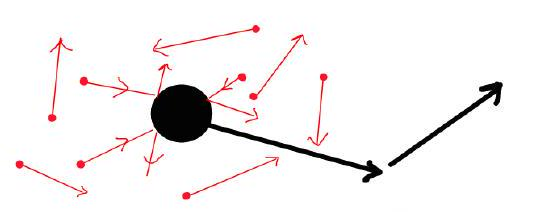
\includegraphics[width=0.5\textwidth]{graphics/2025_10_17_1e406b49946272086d2dg-10}
\end{figure}
\begin{itemize}
  \item Fluid particles at temp T
  \item mesoscopic particle
\end{itemize}
\begin{DispWithArrows}[displaystyle, format=c]
  $m \ddot{\vec{x}}(t)=\vec{F}_{\text { ext }}(\vec{x}(t))+\sum_{i}^{N} i \vec{F}\left(\vec{x}(t)-\vec{x}_{i}(t)\right)$
\end{DispWithArrows}
where $\vec{F}_{\text { ext }}$ is an external force that may (or not) be
described by a potential, where the i-th particle exerts on susp. particle a
force $\bar{F}\left(\bar{x}-\overline{x_{i}}\right)$. As $N \simeq N_{A}$
(Avogadro number), it is pointless to integrate eq. (18). It's more appropriate
to treat the medium particles in an effective way, like an effective force
acting on the susp. particle. Thus
\begin{DispWithArrows}[displaystyle, format=c]
  $\sum_{i}^{N} i \vec{F}\left(\vec{x}(t)-\vec{x}_{i}(t)\right) \simeq \vec{F}_{\text { aver }}+\vec{F}_{\text { noise }}$
\end{DispWithArrows}
As the mesoscopic particle collides with the smaller fluid particles there is
viscous damping generated by the collisions in the fluid. If the velocity of the
particle isn't too large we can approximate
$\vec{F}_{\text { aver }}=-\gamma \vec{v}=-\gamma \dot{\vec{x}}, \gamma$ being the
damping coefficient. From hydrodynamics, we can set $\gamma=6 \pi \eta R$,
$\eta$ being the viscosity and $R$ the Brownian particle's radius.
We also assume that all fluid particles have independent motions and every
particle's movement is independent on different time intervals (if not too
small).

Also, if there is a time interval $\tau$ (much smaller of time intervals of
observation $\Delta t$) large enough that in any two successive time intervals
$\tau$ the motions of the mesoscopic particle can be considered independent
events, then we can effectively approximate $\vec{F}_{\text { noise }}$ as a
stochastic process that is proportional to a Brownian motion.
For simplicity, let's consider the 1-d case with no external forces. So from
(18)
\begin{DispWithArrows}[displaystyle, format=c]
  $m \ddot{x}=-\gamma \dot{x}+\sigma \xi(t)$
\end{DispWithArrows}
where $\langle\xi\rangle=0$ and
$\left\langle\xi(t) \xi\left(t^{\prime}\right)\right\rangle=\delta\left(t-t^{\prime}\right)$.
Notice that this process is non-Markovian. Let's multiply both sides by $x$,
then
\begin{DispWithArrows}[displaystyle, format=c]
  $m x \frac{d}{d t} \dot{x}=-\gamma x \dot{x}+\sigma x \xi_{t}$
\end{DispWithArrows}
Since $\frac{d^{2}}{d t^{2}} x^{2}=2\left(\dot{x}^{2}+x \ddot{x}\right)$, then
\begin{DispWithArrows}[displaystyle, format=c]
  $\frac{m}{2} \frac{d^{2}}{d t^{2}}\left(x^{2}\right)-m \dot{x}^{2}=-\frac{\gamma}{2} \frac{d}{d t}\left(x^{2}\right)+\sigma x \xi_{t}$
\end{DispWithArrows}
Take the average of both sides and use Itô prescription:
\begin{DispWithArrows}[displaystyle, format=c]
  $\frac{m}{2} \frac{d^{2}}{d t^{2}}\left\langle x^{2}\right\rangle-m\left\langle\dot{x}^{2}\right\rangle=-\frac{\gamma}{2} \frac{d}{d t}\left\langle x^{2}\right\rangle$
\end{DispWithArrows}
Because of the equipartition theorem in classical mechanics
\begin{DispWithArrows}[displaystyle, format=c]
  $\frac{m}{2}\left\langle\dot{x}^{2}\right\rangle=\frac{1}{2} k_{B} T$
\end{DispWithArrows}
$k_{B}$ : Boltzmann's constant
hence T: absolute temperature
\begin{DispWithArrows}[displaystyle, format=c]
  $m \frac{d^{2}}{d t^{2}}\left\langle x^{2}\right\rangle+\gamma \frac{d}{d t}\left\langle x^{2}\right\rangle=2 k_{B} T$
\end{DispWithArrows}
Define $y(t)=\frac{d}{d t}\left\langle x^{2}\right\rangle$, then (19b) becomes
\begin{DispWithArrows}[displaystyle, format=c]
  $m \dot{y}+\gamma y=2 k_{B} T$
\end{DispWithArrows}
Whose solution is
$y(t)=c e^{-\frac{\gamma}{m} t}+\frac{2 k_{B} T}{\gamma}$ and $c$ is an
arbitrary constant.
In suspended particles $\frac{m}{\gamma} \simeq 10^{-8} \mathrm{sec}$, which on
temporal scales of observation is a tiny time. Hence for
$t \gg 10^{-8} \mathrm{sec}, y \simeq \frac{2 k_{B} T}{\gamma}$ and
\begin{DispWithArrows}[displaystyle, format=c]
  $\frac{d}{d t}\left\langle x^{2}\right\rangle \simeq \frac{2 k_{B} T}{\gamma}$
\end{DispWithArrows}
so
\begin{DispWithArrows}[displaystyle, format=c]
  $\left\langle x^{2}(t)\right\rangle-\left\langle x_{0}^{2}\right\rangle=\frac{2 k_{B} T}{\gamma} t \text { for } t \gg 10^{-8} \mathrm{sec}$
\end{DispWithArrows}
linear increase of the mean square deviation.
This reminds us of the simple Brownian motion. Indeed, let's start from
\begin{DispWithArrows}[displaystyle, format=c]
  $\dot{x}=\sqrt{2 D} \xi_{t} \text { or } d x=\sqrt{2 D} d B(t)$
\end{DispWithArrows}
which leads to the diffusive equation
\begin{DispWithArrows}[displaystyle, format=c]
  $\frac{\partial}{\partial t} p(x, t)=D \frac{\partial^{2}}{\partial x^{2}} p(x, t) \quad D \text { is diffusivity }$
\end{DispWithArrows}
From (21) $x(t)=x_{0}+\sqrt{2 D} B(t)$ and
\begin{DispWithArrows}[displaystyle, format=c]
  $\left\langle x^{2}\right\rangle=\left\langle x_{0}^{2}+2 x_{0} \sqrt{2 D} B(t)+2 D B(t)^{2}\right\rangle=x_{0}^{2}+2 D t$
\end{DispWithArrows}
diffusion law

By comparing eq. (20) and (22), we obtain
\begin{DispWithArrows}[displaystyle, format=c]
  $D=\frac{k_{B} T}{\gamma}$
\end{DispWithArrows}
Einstein's relation

This is the first and simplest example of fluctuation-dissipation theorem.

\subsection*{Obs:}
\begin{enumerate}
  \item Eq. (23) tells how we should choose the diffusivity if we want to
    interpret physically the mesoscopic particle as a free particle within an
    equilibrium thermal bath at temper. T.
  \item $D$ does not depend on initial conditions, or the nature of interactions
    between the fluid particles and the Brownian particle, all we need to know is
    that the system is at equilibrium in a system where general behavior is
    summarized by the damping constant $\gamma$. (We captured some universal
    behavior here!).
  \item From the diffusion law in eq. (22) one can measure $D$, hence we can give
    an estimate of $k_{B}$ and $N_{A}=\frac{R}{k_{B}}$, the Avogadro number ($R$
is the gas constant). This is what Einstein suggested in his 1905 pioneering
    work on Brownian motion.
  \item This interpretation is straightforward if we start from eq. (19) with
    $\sigma=\sqrt{2 \gamma k_{B} T}$ and then take the limit
    $\frac{m}{\gamma} \rightarrow 0$ which is called the overdamped limit:
\end{enumerate}
\begin{DispWithArrows}[displaystyle, format=c]
  $\frac{m}{\gamma} \ddot{x}=-\dot{x}+\frac{\sqrt{2 \gamma k_{B} T}}{\gamma} \xi_{t} \xrightarrow{m / \gamma \rightarrow 0} \quad \dot{x}=\sqrt{2 \frac{k_{B} T}{\gamma}} \xi_{t}$
\end{DispWithArrows}
overdamped Langevin equation